Hallo.

Da in der vergangenen Session sehr angewandt was in den Sessions zuvor drauf geschafft wurde erschien es mir sinnvoll,
sich nochmal die wichtigsten Gleichungen und ihre Zusammenhänge auf zu schreiben. Now this:

Der pV-Nerd:
\begin{equation}
    pV=nRT
\end{equation}
Der pV-Nerd ist eine Zustandsgleichung. Beschreibt also den derzeitigen Zustand eines (idealen) Gases. Hier stehen \(p\)
für Druck, \(V\) für Volumen, \(n\) die Teilchenzahl, \(R\) für die universelle Gaskonstante mit \(Avogadro \cdot Boltzmann\)
und \(T\) für die Temperatur des Gases.

Arbeit vom oder am Gas:
\begin{figure}[h]
    \centering
    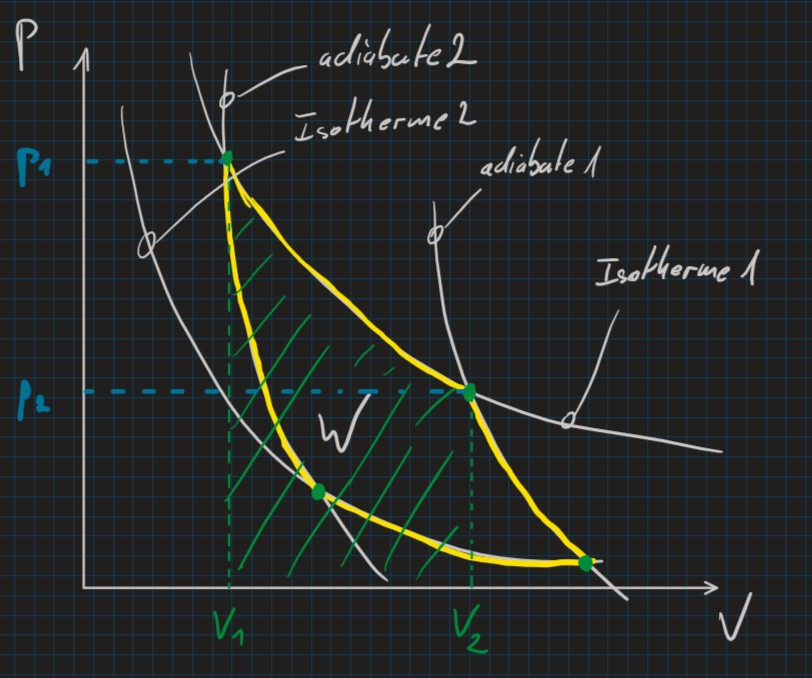
\includegraphics[width=0.5\textwidth]{entries/8/pVwork.jpg}
    \caption{Druck-Volumen-Diagram. Gelb: durchlaufene Zustandsänderung. Grün: aufgewandte Arbeit während der Zustandsänderung (hier exemplarisch entlang der Isotherme 1 von \(V_1\) nach \(V_2\)). Auf dem Weg nach links wird Arbeit am System verrichtet, nach rechts verrichtet das System Arbeit.}
    \label{fig:pVwork}
\end{figure}
Wie in Abbildung \ref{fig:pVwork} ersichtlich entspricht die Arbeit bei der Änderung des Zustandes eines Systems gerade
der Fläche unterhalb des abgetragenen Weges innerhalb des pV-Diagrams. Das Vorzeichen ist hierbei abhängig von der Richtung
in die abgetragen wird.
\begin{align}
    &W = \int_{V_1}^{V_2} p(V) \,\mathrm{d}V = nRT\ln{\frac{V_2}{V_1}} && &\text{Isotherm}\\
    &W = \int_{T_1}^{T_2} nC_{mv} \,\mathrm{d}T = nC_{mv}\Delta T && &\text{Adiabat}
\end{align}
Weiter ist im Falle der adiabatischen Zustandsänderung folgender Zusammenhang hilfreich
\begin{equation}
    T_{wärmer}V_2^{\kappa -1} = T_{kälter}V_3^{\kappa -1}
    \label{eq:adia1}
\end{equation}
\begin{equation}  
    T_{kälter}V_4^{\kappa -1} = T_{wärmer}V_1^{\kappa -1}
    \label{eq:adia2}
\end{equation}
Gleichung \ref{eq:adia1} und \ref{eq:adia2} geben mit etwas Mathemagie (umstellen, proportionalitäten ausnutzen, ...)
(wir sind immernoch bei der adiabatischen Zustandsänderung)
\begin{equation}
    \frac{V_3}{V_4} = \frac{V_2}{V_1}
\end{equation}

\begin{figure}[h]
    \centering
    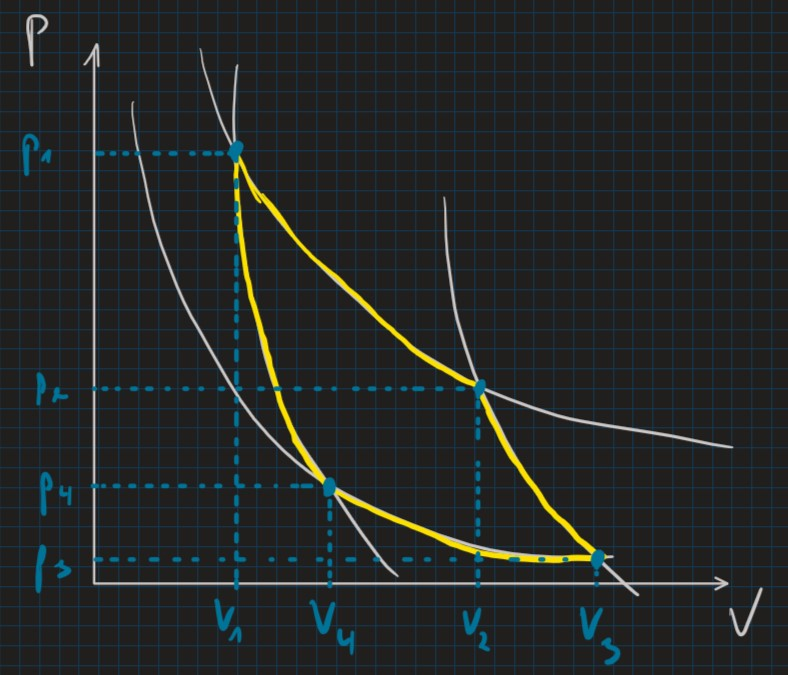
\includegraphics[width=0.5\textwidth]{entries/8/carnot.jpg}
    \caption{Skizzierter Kreisprozess nach Carnot. Blau: Anfangs- und Endzustände}
    \label{fig:carnot}
\end{figure}

Zuletzt - aus den allgemeinen Zusammenhängen der Entropie\textbf{änderung} mit
\begin{equation}
    \Delta S(T,V) = S_0 (T_0 ,V_0 ) + N_A k \ln{\biggl(\frac{T}{T_0}^{\frac{3}{2}} \cdot \frac{V}{V_0}\biggr)}
\end{equation}
\begin{center}
    und
\end{center}
\begin{equation}
    \Delta S(T,p) = S_0 (T_0 ,p_0 ) + N_A k \ln{\biggl(\frac{T}{T_0}^{\frac{5}{2}} \cdot \frac{p}{p_0}\biggr)}
\end{equation}
lassen sich für die verschiedenen Zustandsänderungen recht einfach die Entropiedeltas ermitteln indem an den entsprechenden
Stellen gekürzt wird (\(S_0 (T_0 ,p_0 )\) bzw. \(S_0 (T_0 ,V_0 )\) habe ich entgegen der Vorlesung gleich null gesetzt, da es ohnehin nur um die
Änderung geht).

\begin{center}
    Voilà :)
\end{center}